\documentclass[12pt]{article}

% General
\usepackage[round]{natbib}
\usepackage{setspace}
\usepackage{geometry}
\usepackage[section]{placeins}
\usepackage[hidelinks]{hyperref}
\usepackage{graphicx}
\usepackage{xcolor}
\usepackage{titlesec}
\usepackage[page]{appendix}
\usepackage{enumerate}

% Tables/Figures
\usepackage{lscape}
\usepackage{booktabs}
\usepackage{rotating}
\usepackage{multirow}
\usepackage{longtable}
\usepackage{caption}
\usepackage{subcaption}
\usepackage{float}
\usepackage{tabularx}
\usepackage{ragged2e}
\newcolumntype{Y}{>{\RaggedRight\arraybackslash}X}
\usepackage{pdflscape}
\usepackage{afterpage}

% Math
\usepackage{amsmath}
\usepackage{amssymb}
\usepackage{amsthm}
\usepackage{mathtools}
\usepackage{dsfont}

\usepackage{tikz}

% \doublespacing
\onehalfspacing
% \singlespacing

% \numberwithin{equation}{section}

\geometry{paper=letterpaper, margin=1in}
\captionsetup{font=small}

% Code
\usepackage{textcomp}
\usepackage{sourcecodepro}
\usepackage{listings}
\definecolor{commentgrey}{gray}{0.45}
\definecolor{backgray}{gray}{0.96}
\lstset{
  basicstyle=\footnotesize\ttfamily, keywordstyle=\footnotesize,
  backgroundcolor=\color{backgray}, commentstyle=\color{commentgrey},
  frame=single, rulecolor=\color{backgray}, showstringspaces=false,
  breakatwhitespace=true, breaklines=true, upquote=true,
  numbers=left, numberstyle=\footnotesize\color{commentgrey}}

%%%%%%%%%%%%%%%%%%%%%%%%%%%%%%%%%%%%%%%%%%%%%%%%%%%%%%%%%%%%%%%%%%%%%%%%%%%%%%
% User-defined LaTeX commands
\DeclareMathOperator{\Var}{Var}
\DeclareMathOperator{\Cov}{Cov}
\DeclareMathOperator{\Corr}{Corr}
\DeclareMathOperator*{\argmax}{arg\,max}
\DeclareMathOperator*{\argmin}{arg\,min}
\DeclarePairedDelimiter{\abs}{\lvert}{\rvert}
\DeclarePairedDelimiter{\norm}{\lVert}{\rVert}
\newcommand*{\expp}[1]{\exp\left(#1\right)}
\newcommand*{\foralls}{\ \forall \ }
\newcommand*{\st}{\text{ s.t. }}
\newcommand*{\E}{\mathbb E}
\newcommand*{\R}{\mathbb R}
\newcommand*{\I}{\mathds{1}}
\newcommand*{\Prob}{\mathbb P}
\newcommand*{\convas}[1]{\xrightarrow{#1}}
\newcommand*{\conv}{\convas{}}
\newcommand*{\cond}{\;\ifnum\currentgrouptype=16 \middle\fi|\;}
\newcommand*{\defeq}{%
  \mathrel{\overset{\makebox[0pt]{\mbox{\normalfont\tiny\sffamily def}}}{=}}}
\newcommand*{\notorth}{\ensuremath{\perp\!\!\!\!\!\!\diagup\!\!\!\!\!\!\perp}}
\newcommand*{\orth}{\ensuremath{\perp\!\!\!\perp}}
\newcommand*{\evalat}{\,\big\rvert}
\newcommand*{\dif}{\,d}
\newcommand*{\difto}[1]{\,d^#1}
\newcommand*{\difbot}[1]{\frac{d}{d#1}}
\newcommand*{\partialbot}[1]{\frac{\partial}{\partial#1}}
\newcommand*{\m}[1]{\textbf{#1}}
\newcommand*{\bmath}[1]{\boldsymbol{#1}}

\newcommand*{\yestag}{\addtocounter{equation}{1}\tag{\theequation}}
\newcommand*{\notaligned}[1]{\noalign{$\displaystyle #1$}}
\newcommand*{\ttilde}{{\raise.17ex\hbox{$\scriptstyle\sim$}}}

\makeatletter
\newsavebox{\mybox}\newsavebox{\mysim}
\newcommand*{\distas}[1]{%
  \savebox{\mybox}{\hbox{\kern3pt$\scriptstyle#1$\kern3pt}}%
  \savebox{\mysim}{\hbox{$\sim$}}%
  \mathbin{\overset{#1}{\kern\z@\resizebox{\wd\mybox}{\ht\mysim}{$\sim$}}}%
}
\makeatother
\newcommand*{\dist}{\sim}
\newcommand*{\distiid}{\distas{\text{i.i.d}}}

\makeatletter
\def\moverlay{\mathpalette\mov@rlay}
\def\mov@rlay#1#2{\leavevmode\vtop{%
   \baselineskip\z@skip \lineskiplimit-\maxdimen
   \ialign{\hfil$\m@th#1##$\hfil\cr#2\crcr}}}
\newcommand*{\charfusion}[3][\mathord]{
  #1{\ifx#1\mathop\vphantom{#2}\fi\mathpalette\mov@rlay{#2\cr#3}}
  \ifx#1\mathop\expandafter\displaylimits\fi}
\makeatother
\newcommand*{\cupdot}{\charfusion[\mathbin]{\cup}{\cdot}}
\newcommand*{\bigcupdot}{\charfusion[\mathop]{\bigcup}{\cdot}}

\newcommand*{\mt}[1]{\text{\normalfont #1}}

\newtheorem{theorem}{Theorem}[section]
\newtheorem{theorem*}{Theorem}
\newtheorem{corollary}{Corollary}[section]
\newtheorem{proposition}{Proposition}[section]
\newtheorem{lemma}{Lemma}[section]

\theoremstyle{definition}
\newtheorem{definition}{Definition}[section]
\newtheorem{definition*}{Definition}
\newtheorem{example}{Example}[section]
\newtheorem*{properties}{Properties}

\newtheoremstyle{algodesc}{}{}{}{}{\bfseries}{.}{ }{}%
\theoremstyle{algodesc}
\newtheorem{algodesc}{Algorithm}
%%%%%%%%%%%%%%%%%%%%%%%%%%%%%%%%%%%%%%%%%%%%%%%%%%%%%%%%%%%%%%%%%%%%%%%%%%%%%%

\newcommand*{\colsquare}[3][-3.5pt]{\tikz[baseline=-0.5ex]\draw[#2, fill=#2] (0,#1) rectangle ++(#3,#3);}%
\definecolor{cmeet}{HTML}{B2DF8A}
\definecolor{cmideast}{HTML}{FDBF6F}
\definecolor{cstaff}{HTML}{A6CEE3}
\definecolor{cpolitics}{HTML}{33A02C}
\definecolor{cterror}{HTML}{E31A1C}
\definecolor{cforeign}{HTML}{FF7F00}
\definecolor{cpress}{HTML}{FB9A99}
\definecolor{chill}{HTML}{6A3D9A}
\definecolor{ccomm}{HTML}{1F78B4}


\begin{document}

\title{Exploring Hillary Clinton's Emails\thanks{STATS 601 final project.}}
\author{
    Leland Bybee, Roger Fan, Ryan Vaughn
}
\date{\today}

\maketitle


\section{Introduction}
From roughly 2008 to 2013, Hillary Clinton and some of her staff used a private family email server for most of he communication. This time period includes her tenure as U.S. Secretary of State, and has therefore become a controversial topic due to the possible security concerns of not using official government servers. Various investigations into the legality and appropriateness of the email server have been launched, and the issue has had/will potentiall have a large effect on Clinton's ongoing presidential campaign.

Due to several Freedom of Information Act (FOIA), the State Department has released the vast majority of the roughly 55,000 pages of emails to the public, leading to an unprecedented opportunity to explore the email usage of a major public figure.

Due to the size of the corpus, reading individual emails in the hope of discovering interesting characteristics is unrealistic. We therefore exploit statistical methods to break this vast analysis problem to a more manageable one, decreasing the scale so that we can more easily apply human and statistical analysis.

In order to tackle this problem, we use classical multi-dimensional scaling and spectral clustering in order to visualize and explore the corpus. We also use a statistical topic model, latent Dirichlet analysis (LDA), in order to identify and analyze the meanings and semantics. Finally, we use the LDA results and other metadata to examine how other covariates, such as email sender and time period sent, are related to the topic of an email.


\section{Data}
The State Department released the raw data in the form of roughly 30,000 pdfs of individual emails from the Clinton server.\footnote{Thanks to Ben Hamner and the Wall Street Journal for making the data processing code (\url{https://github.com/benhamner/hillary-clinton-emails}) and email pdfs (\url{http://graphics.wsj.com/hillary-clinton-email-documents/}) available, respectively.} We first process the pdfs to extract the raw text.\footnote{We used \texttt{pdftotext}, an open-source program used to extract text from pdf files.} From the raw email text, email headers and forward/response information are stripped, leaving only the subject line and body text.

All of our methods use a bag-of-words model, so from this raw data we construct a document term matrix containing vectors of word counts. Some standard data cleaning for text data is also performed, including the removal of punctuation and email addresses, word stemming (combining words with common roots, e.g. calling and called), and removing extremely common words (i.e. stop words) and extremely rare words (words that appear in less than 0.1\% of emails).

After this processing, we are left with a dataset of roughly 28,000 emails and a total vocabulary of over 3,000 words. Note that each word count vector is extremely sparse, so we need statistical methods that can apply in a sparse coordinate setting. Also, methods that can efficiently exploit this sparseness to reduce computation are preferred.


\section{Visualization}
Due to the large size and high dimensionality of the data, we must apply some dimensionality reduction in order to effectively visualize it. We therefore apply classical multi-dimensional scaling, which attempts to place each point in a much smaller dimension such that pairwise distances are preserved.

However, we expect standard Euclidean distance to poorly capture the actual relationships between vectors of word counts. In particular, Euclidean distance is affected by the total number of words, two emails with the exact same word distribution that differ in length could have a very large distance between them. In order to better capture pairwise relationships, we will use a distance metric based on the angles between vectors.

We define the cosine similarity between word frequency vectors $V$ and $W$ to be the cosine of the angle between the two vectors, calculated as
\begin{equation} \label{eq:cos_sim}
\cos(\phi) = \frac{\langle V, W \rangle}{\norm{V}\norm{W}}
\end{equation}
Since counts must be nonnegative, note that $\phi \leq \pi/2$. This implies that the cosine similarity is always between 0 and 1, with 0 corresponding to vectors that are multiples of each other and 1 corresponding to orthogonal vectors (i.e. no shared words). So we can define the cosine distance as
\begin{equation} \label{eq:cos_dist}
d(V, W) = 1 - \cos(\phi) = 1 - \frac{\langle V, W \rangle}{\norm{V}\norm{W}}
\end{equation}

Using this measure of distance, we can construct a distance matrix $D$ and apply MDS. The results for an 8,000 email subset are shown in Figure~\ref{fig:cluster}, plotted in both two and three dimensions. We can see several interesting patterns. The vast majority of emails (roughly 5,000) are contained in the main central grouping, with two large groupings that extend away. Besides these two ``arms,'' however, it is difficult to visually identify other significant structures.

\begin{figure}[htbp] \centering
  \begin{subfigure}[t]{.7\linewidth}
    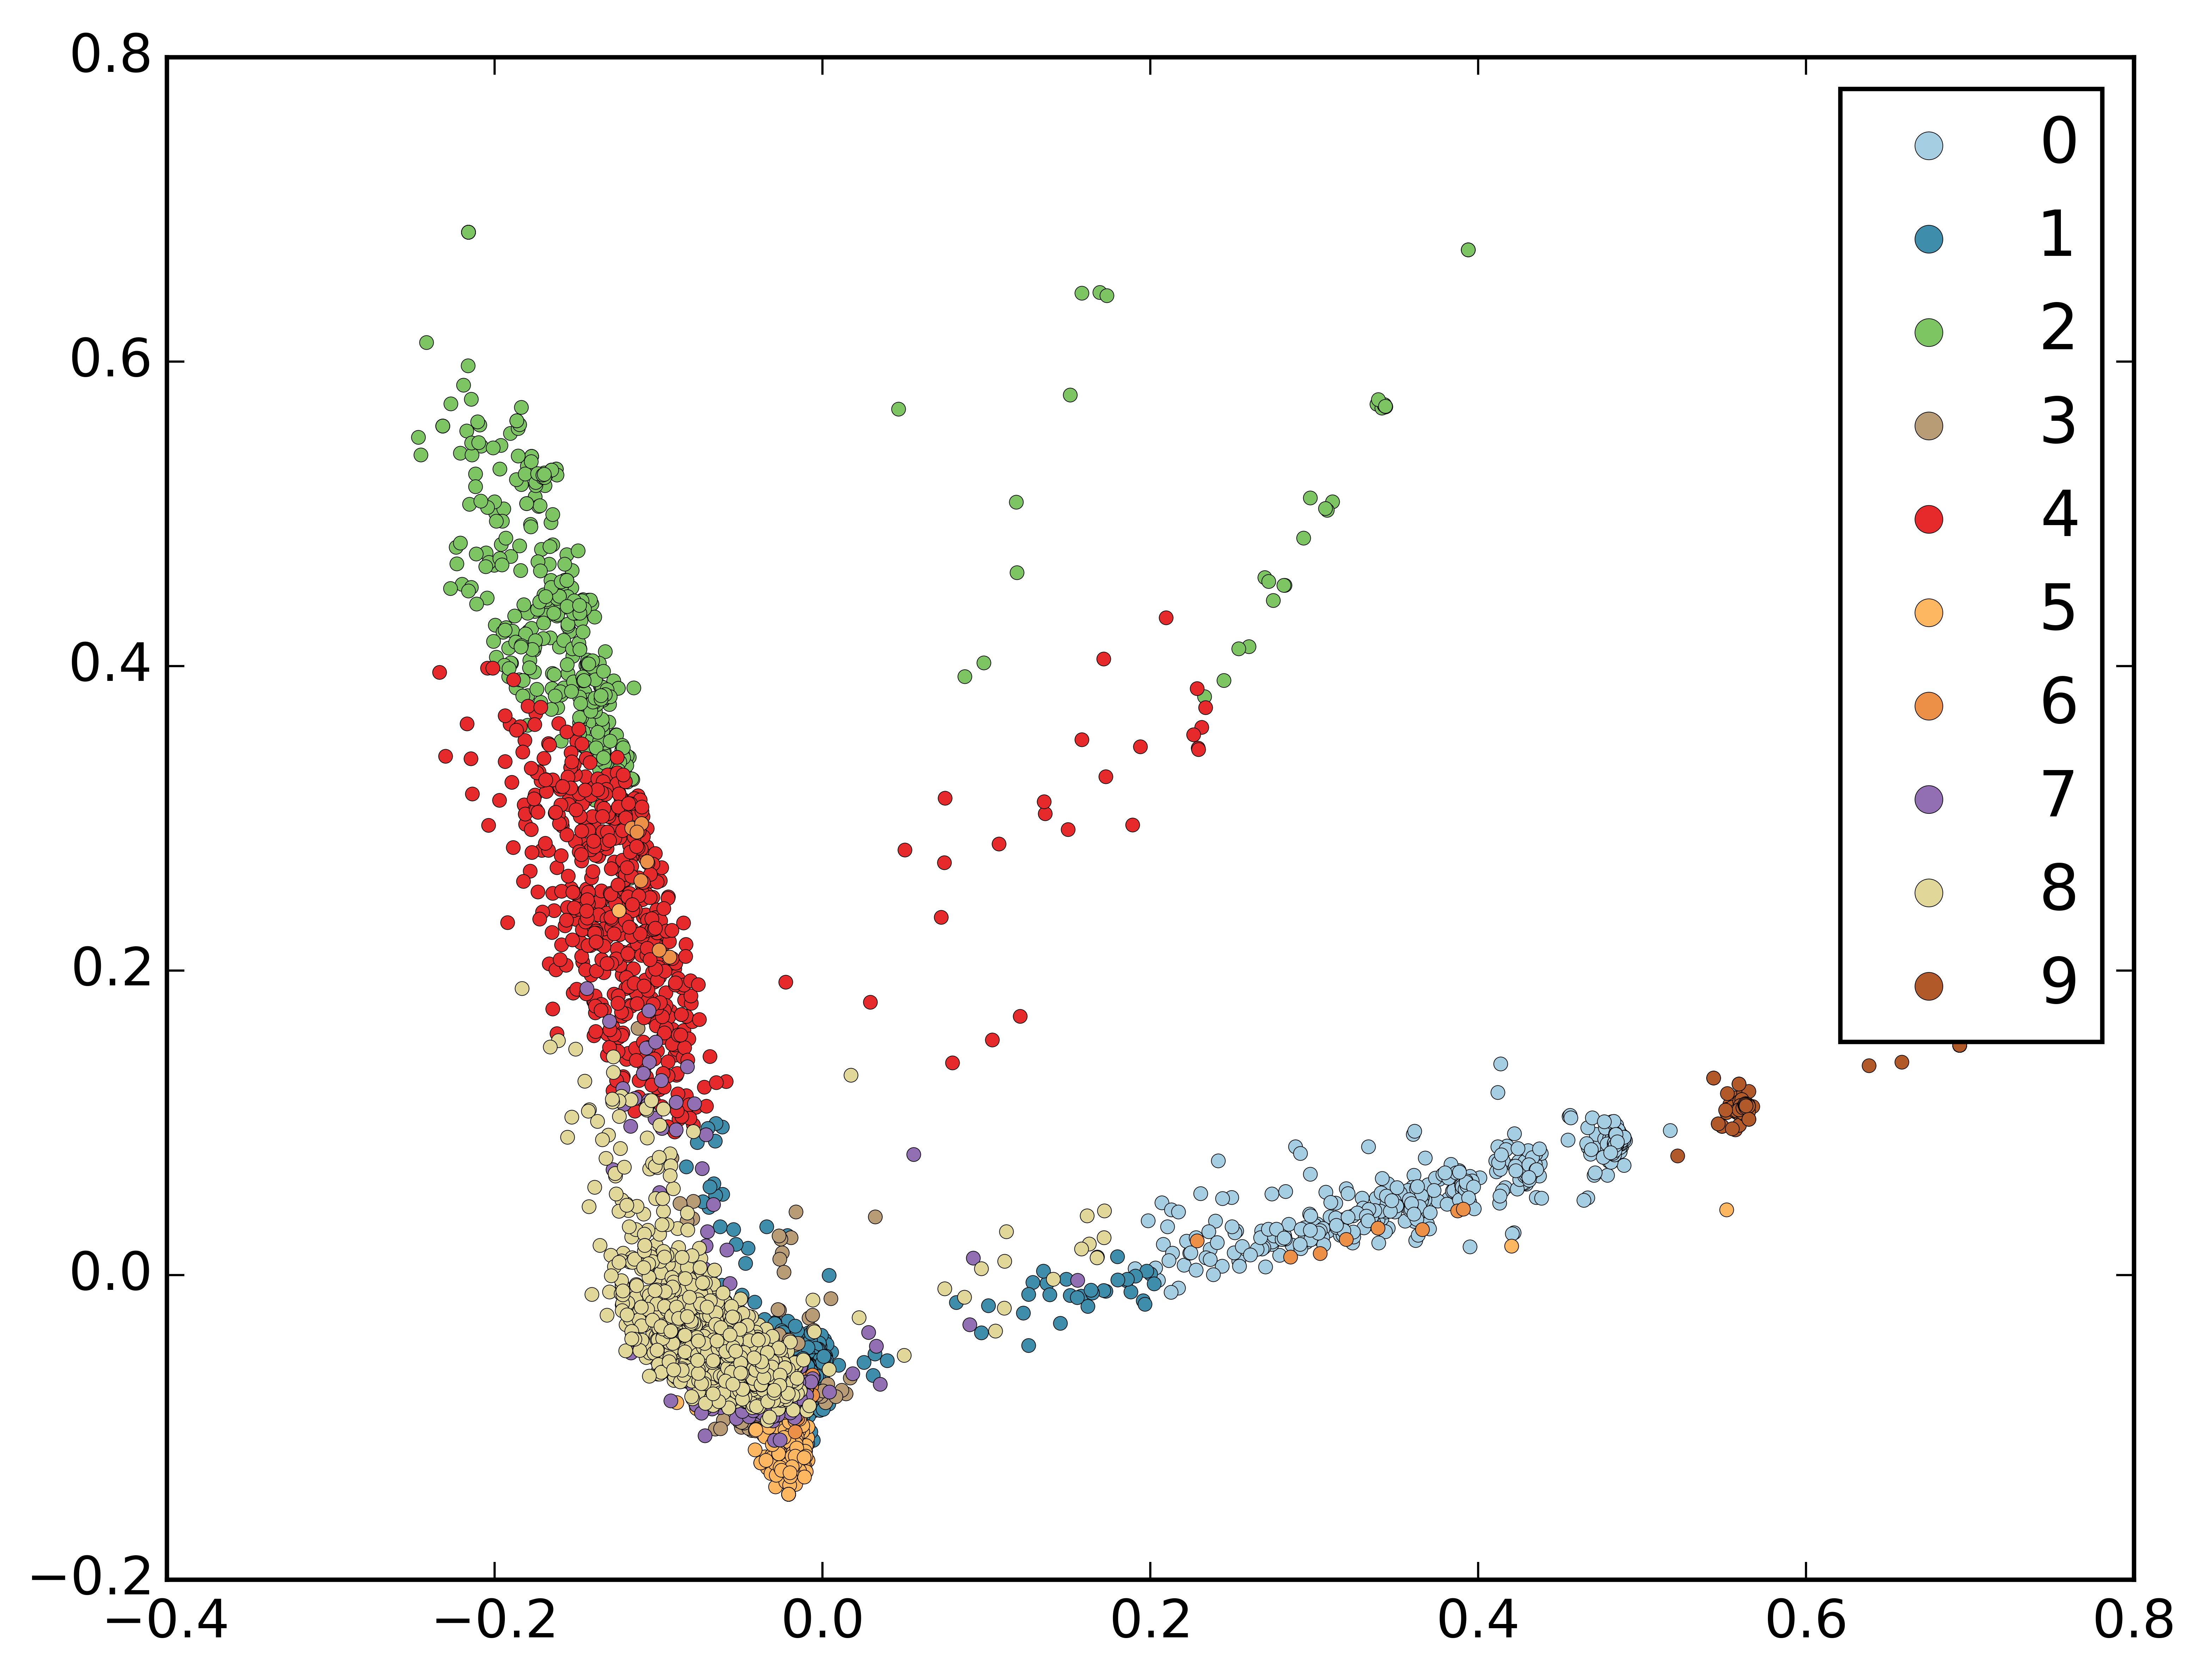
\includegraphics[width=\linewidth]{../images/mds_2d_cluster.png}
    \caption{2 Dimensions} \label{fig:cluster:2d}
  \end{subfigure}
  \begin{subfigure}[t]{.7\linewidth}
    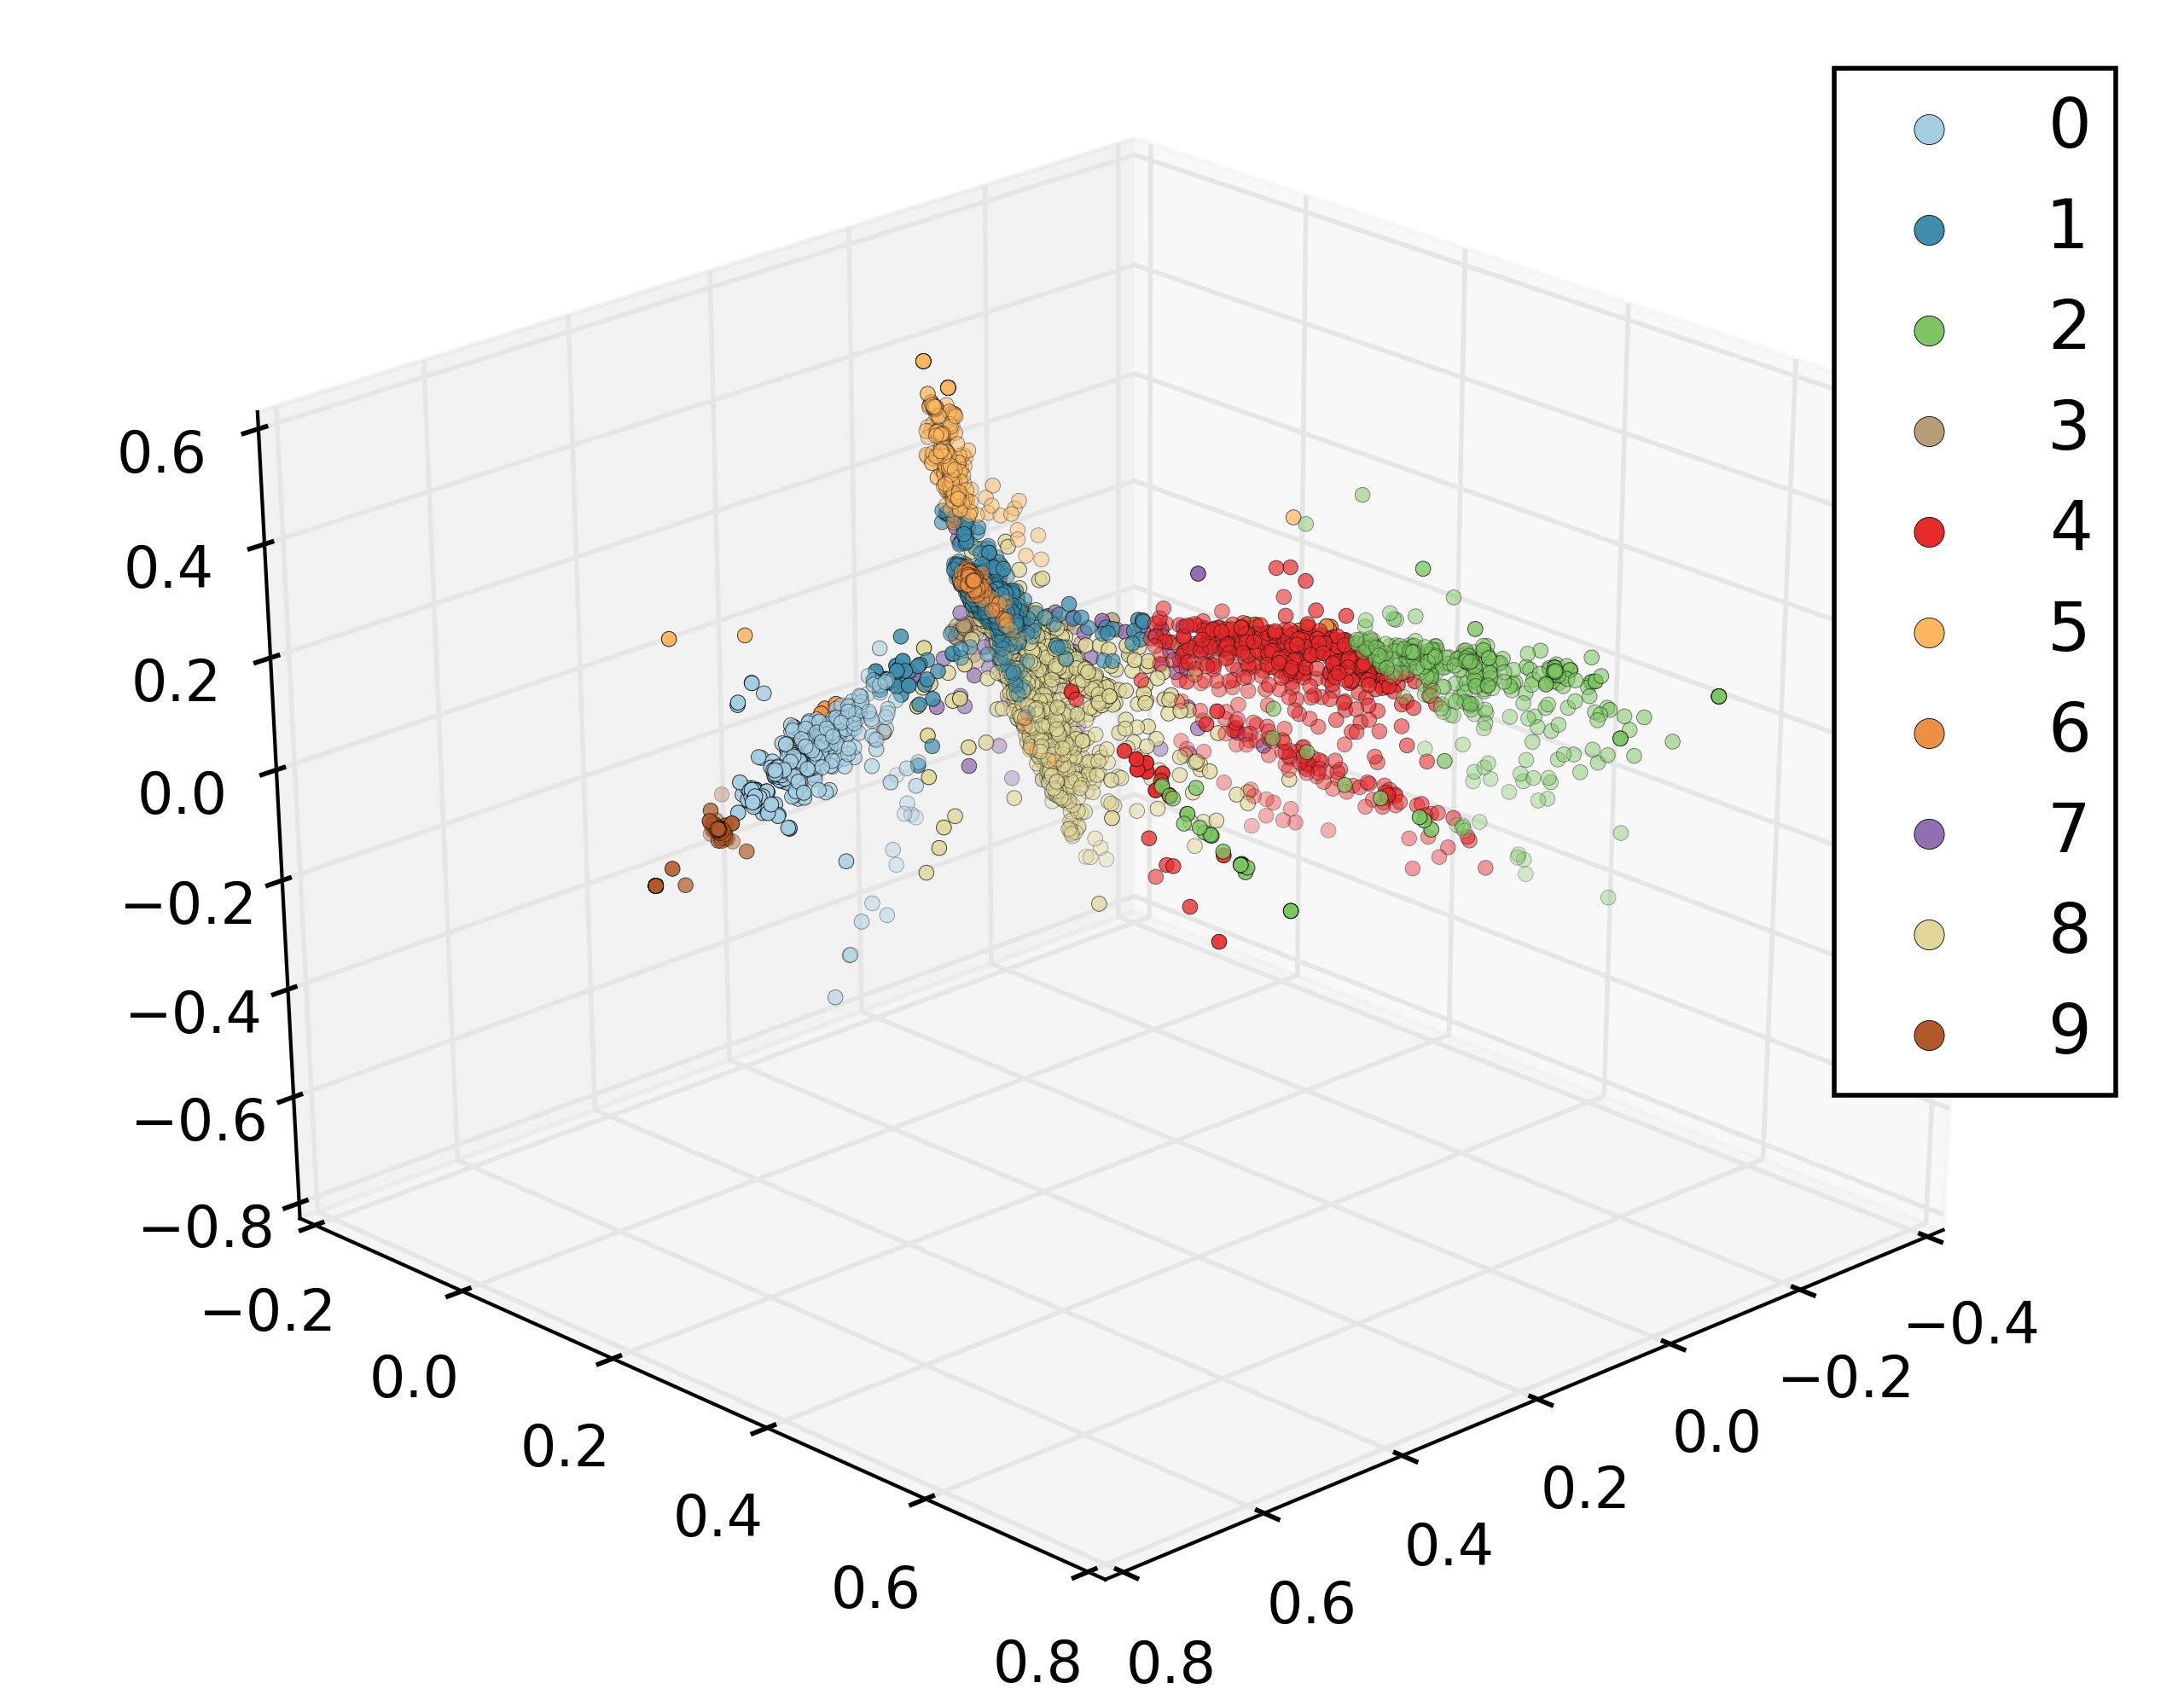
\includegraphics[width=\linewidth]{../images/mds_3d_cluster_1.png}
    \caption{3 Dimensions} \label{fig:cluster:3d}
  \end{subfigure}
  \caption{Visualization of a 8,000 email subset using classical multi-dimensional scaling and with coloring according to the results from spectral clustering. The similarity and distance metrics used for spectral clustering and MDS, respectively, are cosine similarity and distance as defined in Equations~\ref{eq:cos_sim} and~\ref{eq:cos_dist}.}
  \label{fig:cluster}
\end{figure}


\subsection{Spectral Clustering}
In order to better identify structure that may exist in the data, we attempt to apply clustering methods. However, it is important to choose an appropriate clustering method due to the high dimensionality and sparse nature of the data. In particular, we expect centroid-based methods such as Gaussian mixture models and $k$-means clustering to perform poorly in this setting.

Spectral clustering, however, exploits the information contained in the pairwise distances (or, equivalently, the similarities) between points. By using pairwise distances, spectral clustering is particularly well-suited to finding clusters that may not necessarily be spherical or ellipsoidal and that may lie along lower-dimensional manifolds.

To actually apply spectral clustering, we first construct the pairwise similarity matrix $S$ using our cosine similarity as defined in Equation~\ref{eq:cos_sim}. We define the degree matrix $D$ to be a diagonal matrix with $D_{ii} = \sum_j S_{ij}$, and construct the symmatrix normalized Laplacian matrix as
\begin{equation} \label{eq:laplacian}
L = I - D^{-1/2} S D^{-1/2}
\end{equation}
Then the eigenvectors corresponding to the smallest $k$ eigenvalues of $L$ are computed and $k$-means clustering is performed on these eigenvectors.

Figure~\ref{fig:cluster} classifies each point according to the results of spectral clustering with $k$ clusters. We can see that many of the cluster correspond to  the visually identifiable structures, including clusters that correspond to each of the ``arms.''

By investigating the individual emails, we can also get a sense of what each cluster consists of. For instance, clusters 2 and 4 consist of emails related to calls and communication. In this arm, those closer to the main central clump contain more conversation, while those farther out are much briefer and directly about the call (e.g. ``I'd like to call tomorrow.''). Cluster 3 consists entirely of ``minis,'' summaries of the days schedule sent to Clinton each morning. Emails from cluster 5 are generally requests to print materials, while those from cluster 6 are forwarded news articles.

In general, it seems that spectral clustering does a good job at identifying emails by their structure, but does not tell us much about the meaning of an email. We can tell that an email is regarding a call or is a news headline by what cluster it is in, but not what that call or headline is about. On a related note, it does not do a good job separating the ``regular'' emails. OVer 5,000 of the 8,000 emails depicted fall into clusters 1 or 8, which essentially consist of all the emails without specific identifiable structure. Ideally we would be able to further classify these emails according to subject matter, but clustering does not seem suited to this task.


\section{Topic Modeling}
Include model description, estimation strategy, and model selection.

\subsection{Interpreting Topics}
Include ``grunt work'' of interpreting topics, topic frequency

\begin{table}[htb] \centering
\begin{tabular}{rcl}
  \toprule
  \colsquare{cterror}{10pt} & Terrorism & 5, 22 \\
  \colsquare{cmideast}{10pt} & Middle East & 6, 18, 19, 27, 29 \\
  \colsquare{cforeign}{10pt} & Foreign Policy & 2, 7, 13, 21, 23, 26 \\
  \colsquare{cpolitics}{10pt} & Politics & 11, 17, 25 \\
  \colsquare{cstaff}{10pt} & Staff & 16, 20 \\
  \colsquare{cpress}{10pt} & Press & 4 \\
  \colsquare{chill}{10pt} & Hillary & 12 \\
  \colsquare{cmeet}{10pt} & Meetings & 1, 9, 10, 24, 28, 30 \\
  \colsquare{ccomm}{10pt} & Common & 3, 8, 14, 15 \\
  \bottomrule
\end{tabular}
\caption{Topic Categorization}
\label{tab:topic_cat}
\end{table}

\begin{table}[htb] \centering
\setlength{\tabcolsep}{1pt}
\begin{tabular}{cccccccccccccccccccccccccc}
  \toprule
  \colsquare[-3pt]{cforeign}{16pt} &
  \colsquare[-3pt]{cmeet}{16pt} &
  \colsquare[-3pt]{cmeet}{16pt} &
  \colsquare[-3pt]{cmeet}{16pt} &
  \colsquare[-3pt]{cmeet}{16pt} &
  \colsquare[-3pt]{cmeet}{16pt} &
  \colsquare[-3pt]{cpress}{16pt} &
  \colsquare[-3pt]{cmeet}{16pt} &
  \colsquare[-3pt]{cmideast}{16pt} &
  \colsquare[-3pt]{cmideast}{16pt} &
  \colsquare[-3pt]{cstaff}{16pt} &
  \colsquare[-3pt]{chill}{16pt} &
  \colsquare[-3pt]{cstaff}{16pt} &
  \colsquare[-3pt]{cpolitics}{16pt} &
  \colsquare[-3pt]{cforeign}{16pt} &
  \colsquare[-3pt]{cmideast}{16pt} &
  \colsquare[-3pt]{cforeign}{16pt} &
  \colsquare[-3pt]{cmideast}{16pt} &
  \colsquare[-3pt]{cterror}{16pt} &
  \colsquare[-3pt]{cmideast}{16pt} &
  \colsquare[-3pt]{cforeign}{16pt} &
  \colsquare[-3pt]{cpolitics}{16pt} &
  \colsquare[-3pt]{cforeign}{16pt} &
  \colsquare[-3pt]{cforeign}{16pt} &
  \colsquare[-3pt]{cpolitics}{16pt} &
  \colsquare[-3pt]{cterror}{16pt} \\
  21 & 1 & 28 & 30 & 10 & 9 & 4 & 24 & 18 & 29 & 16 & 12 & 20 &
  17 & 13 & 19 & 23 & 27 & 22 & 6 & 2 & 25 & 26 & 7 & 11 & 5 \\
  \midrule
  \multicolumn{13}{l}{Most Frequent} & \multicolumn{13}{r}{Least Frequent} \\
  \bottomrule
\end{tabular}
\setlength{\tabcolsep}{6pt}
\caption{Primary Topic Frequency}
\label{tab:topic_freq}
\end{table}


\subsection{Types of Topics}
Talk about structural, common word, and semantic topics, including ``interesting'' vs. ``non-interesting'' topics, discuss strengths of model in comparison to MDS

\subsection{Topic Analysis}
Analyze some specific topics, compare use over time and how it correlates with related events


\section{Email Sender Prediction}
Talk about the who says what table

\subsection{Multinomial Logistic Regression}
Quickly describe model and discuss results

\begin{figure}[htb] \centering
  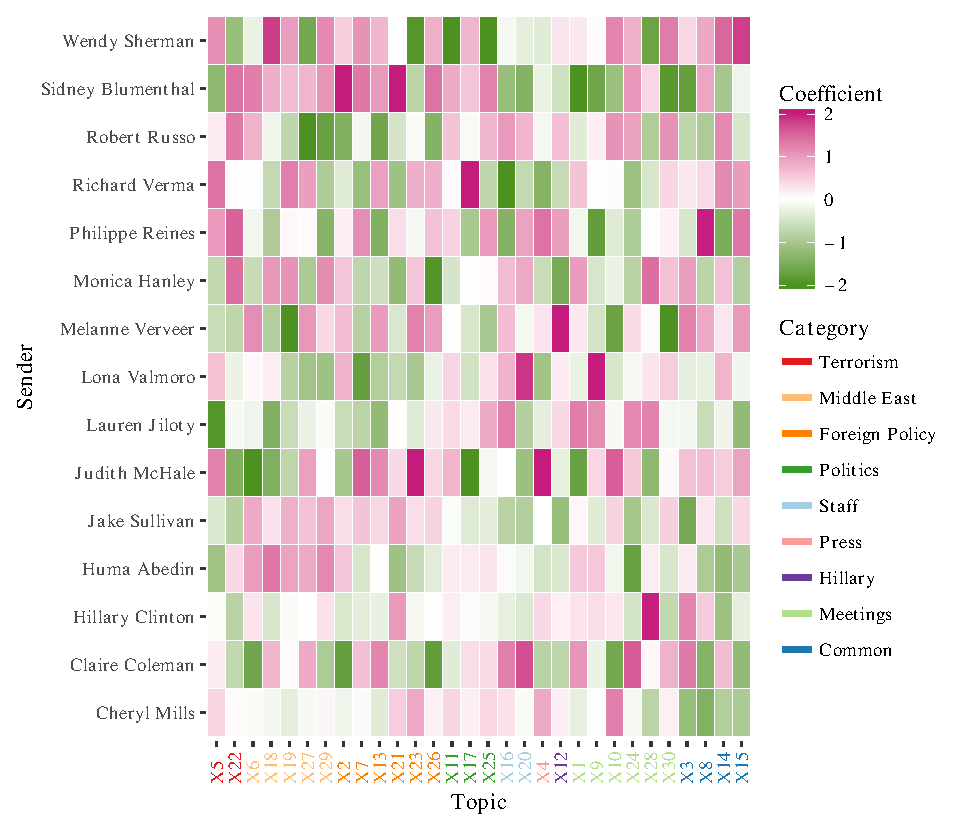
\includegraphics[width=0.95\linewidth]{../images/coefficients.pdf}
  \caption{Normalized coefficients from a multinomial logistic regression of email sender on LDA topic proportions.}
  \label{fig:coefficients}
\end{figure}


\section{Conclusion}



\end{document}
